%%%%%%%%%%%%%%%%%%%%%%%%%%%%%%%%%%%%%%%%%%%%%%%%%%%%%%%%%%%%%%%%%%%%%%%%%%%%%%%%
%2345678901234567890123456789012345678901234567890123456789012345678901234567890
%        1         2         3         4         5         6         7         8

\documentclass[letterpaper, 10 pt, conference]{ieeeconf}  % Comment this line out
                                                          % if you need a4paper
%\documentclass[a4paper, 10pt, conference]{ieeeconf}      % Use this line for a4
                                                          % paper

\IEEEoverridecommandlockouts                              % This command is only
                                                          % needed if you want to
                                                          % use the \thanks command
\overrideIEEEmargins
% See the \addtolength command later in the file to balance the column lengths
% on the last page of the document



% The following packages can be found on http:\\www.ctan.org
%\usepackage{graphics} % for pdf, bitmapped graphics files
%\usepackage{epsfig} % for postscript graphics files
%\usepackage{mathptmx} % assumes new font selection scheme installed
%\usepackage{times} % assumes new font selection scheme installed
\usepackage{amsmath} % assumes amsmath package installed
%\usepackage{amssymb}  % assumes amsmath package installed
\usepackage{graphicx}

%% Macros
\def\trainingset{\{x_i,y_i\}_{i=0}^{N-1}}
\def\pnmlSingle{\max_{\theta} P_\theta (y_N|x_N, z^N)}

\title{\LARGE \bf
Predictive Normalize Likelihood for Least Squares Predictor: Toward better understanding of Model Generalization
}

%\author{ \parbox{3 in}{\centering Huibert Kwakernaak*
%         \thanks{*Use the $\backslash$thanks command to put information here}\\
%         Faculty of Electrical Engineering, Mathematics and Computer Science\\
%         University of Twente\\
%         7500 AE Enschede, The Netherlands\\
%         {\tt\small h.kwakernaak@autsubmit.com}}
%         \hspace*{ 0.5 in}
%         \parbox{3 in}{ \centering Pradeep Misra**
%         \thanks{**The footnote marks may be inserted manually}\\
%        Department of Electrical Engineering \\
%         Wright State University\\
%         Dayton, OH 45435, USA\\
%         {\tt\small pmisra@cs.wright.edu}}
%}

\author{Koby Bibas and Meir Feder $^{*}$% <-this % stops a space
\thanks{$^{*}$School of Electrical Engineering,
	Tel Aviv University, Tel Aviv, 6887801, Israel}
}

\begin{document}



\maketitle
\thispagestyle{empty}
\pagestyle{empty}


%%%%%%%%%%%%%%%%%%%%%%%%%%%%%%%%%%%%%%%%%%%%%%%%%%%%%%%%%%%%%%%%%%%%%%%%%%%%%%%%
\begin{abstract}
Universal supervised learning is considered from an information theoretic point of view following the universal prediction approach. The information
theoretical approach naturally uses the self-information loss or log-loss. We consider the standard " learning where prediction is done on a test sample once the entire training data is
observed, and the individual setting where the features and labels, both in the training and test,
are specific individual quantities.
Our results provide universal learning schemes that compete with a genie", depned below,
that knows the true test label. In particular, it is demonstrated that the main proposed scheme,
termed Predictive Normalized Maximum Likelihood (pNML), is a robust learning solution
that outperforms the current leading approach based on Empirical Risk Minimization (ERM).
Furthermore, the pNML construction provides a pointwise indication for the learnability of a
specic test challenge with the given training examples. The scheme and its advantages are
shown in some examples.
\end{abstract}


%%%%%%%%%%%%%%%%%%%%%%%%%%%%%%%%%%%%%%%%%%%%%%%%%%%%%%%%%%%%%%%%%%%%%%%%%%%%%%%%




%% main text
\section{Introduction} \label{Introduction}
In machine learning the most common tasks are classification and regression. In classification, given train set which consist N pairs $z^N=\{(x_i, y_i)\}_{i=0}^{N-1}$ where $x \in \mathcal{X}$ is the data and $y \in \mathcal{Y}$ are the labels for which $\mathcal{Y}$ is a finite set. The goal is to predict the label $y_N$ of unseen data $x_N$. The regression task setting are the same as the classification except that the label space $\mathcal{Y}$ is infinite and continuous.
In order to evaluate the performance of some predictor $q$ on the test sample $(x_N, y_N)$, we need to use loss function  $\mathcal{L}$. Using the framework of the information theory field, we consider the log-loss
\begin{equation}
 \mathcal{L}(q,x_N,y_N) = -P(y_N|x_N)\log {q(y_N|x_N}).
\end{equation}
The best predictor is one who has the minimal loss for all test samples.

The main settings of the way the pairs $\{x,y\}$ are generated are the stochastic setting, the Probably Approximately Correct (PAC) setting and individual settings. In the stochastic setting the data and labels are assumed to be generated from probabilistic source, i.e. there is probabilistic assignment $P_\theta(y|x)$ from a set of hypotheses class $\theta \in \Theta$ and our goal is to find it. 

The concept of PAC was established in  \cite{valiant1984theory}.
In this setting, the data samples assumed to be generated independently from some source $P(x,y)=P(x)P(y|x)$, however, unlike the stochastic setting, $P(y|x)$ is not necessarily a member of the hypotheses class.
The purpose in this setting is to design an algorithm that attains, with very high probability over the possible training sets, a loss which is almost that of the best hypothesis in the class. 

In this paper we consider the scenario of the individual setting. 
In the individual setting the assumption that the data and labels were created by  probabilistic mechanism is not longer valid and finding assignment of y given x is therefore impossible. 
The goal now becomes to be as good as possible as a learner who has information about the training set along with the label of the test sample. 
We call this kind of learner a Genie \cite{feder1992universal}. The Genie has some constraints: it's restricted to be a member of a hypothesis class $\{P_\theta(y_N|x_N,y_N,z^N)\ , \ \theta \in \Theta \}$.  
In addition, it has no knowledge about which of the sample it is going to be tested on. 
The log-loss difference between our learner and the Genie is known as the regret:
\begin{multline} \label{eq:genie_regret}
R(\theta, q, x_N, z^N) = \\ \sum_{y \in \mathcal{Y}} P_\theta(y_N|x_N,y_N,z^N) log \frac{P_\theta(y_N|x_N,y_N,z^N)}{q_(y_N|x_N, z^N)} 
\end{multline}

The most common approach of generating a leaner is the Empirical Risk Minimization (ERM) \cite{vapnik1992principles}. Given a training set, a predictor is chosen from a predictors class $\{P_\theta(y|x) , \quad \theta \in \mathcal{\theta}\}$ in a way it minimizes the training set error 
\begin{equation}
Q(y|x) = \min_\theta \frac{1}{N}\sum_{i=0}^{N-1}  l(y_i,P_\theta(y_i|x_i)).
\end{equation}
The underline assumption of the ERM approach is that the the problem setting is stochastic and that training data are independent.

In this paper we use the Predictive Normalized Likelihood (PNML). The PNML is the solution of the minmax problem of equation \ref{eq:genie_regret} \cite{shtar1987universal}
\begin{equation}
Q_{\textit{PNML}}(\cdot|x_N,z^N) = \underset{q}{\textit{argmin }}\underset{y_N}{\textit{max }} R(\theta, q, x_N, z^N)
\end{equation}
and the solution is 
\begin{equation} \label{eq:pnml}
Q_{PNML}(y_N|x_N,z^N)=\frac{\pnmlSingle}{\sum_{y\in \mathcal{Y}} \pnmlSingle}.
\end{equation}
In order to obtain the PNML predictor the following procedure is executed: we assume the label of the test data is known, fit a learner to it and predict the assumes label by it. We repeat the process for all possible label. In the end we normalize the probabilities from each label and return the PNML estimator.

The regret in this case is the normalization factor of the PNML
\begin{equation} \label{eq:pnml_regret}
R(Q_{\textit{PNML}, x_N, z^N}) = \log \left\{ \sum_{y\in \mathcal{Y}} \pnmlSingle \right\}
\end{equation}

The problem of on-line learning, especially in the individual setting has been recently analyzed in Fogel
and Feder (2017). in this paper we focus on the standard batch supervised learning problem, in the individual setting. The paper is organized and presents the results in
the following manner.

This paper deals with the least squares model family, which is a standard approach in regression analysis \cite{lawson1995solving}. In this approach, the overall solution minimizes the sum of the squares of the residuals made in the results of every single equation. For the least squares family, we have derived an analytic solution for the PNML from equation \ref{eq:pnml}.

The main contributions of this paper are:
\begin{itemize}
  \item Applying the PNML solution to the Least Squares predictors family.
  \item Analyze for which test samples the proposed PNML estimator can generalize. 
  \item ??
\end{itemize}

The paper outline is as follows.
Section \ref{sec:formal_problem_def} introduces the setting and the goal of the regression problem. In section \ref{sec:PNML_eval} the evaluation of the PNML is presented and analyses. In depth analyze of the learnable space is shown in \ref{sec:learnable_space}. The simulation of the PNML and its regret on estimating polynomial coefficients is shown in section \ref{sec:simulation} and the conclusion and future work is in section \ref{sec:conclusion}.



\section{Formal Problem Definition} \label{sec:formal_problem_def}
Given N pairs of data and labels $\{x_i, y_i\}_{i=0}^{N-1}$ where $x_i \in R^M, y\in R$ are deterministic. Our model takes the form:
\begin{equation}
y_i=x_i^T \theta + e_i
\end{equation}
where $\theta \in R^M$ are the learnable parameters and $e \in R$ is white Gaussian noise with variance of $\sigma$. 
Our goal is to predict $y_N$ based on a new data sample $x_N$:
\begin{equation}
y_N = x_N^T \theta + e_N.
\end{equation}
In this case $y_N$ has normal distribution that depends on the learnable parameters $\theta$ 
\begin{equation}
P_{\theta}(y_N) 
=\frac{1}{\sqrt[]{2\pi\sigma^2}}exp\left\{-\frac{1}{2\sigma^2}\big(y_N- x_N^T\theta \big)^2\right\}  \\
\end{equation}
We consider the $\theta$ to be a member of hypothesis class $\Theta$, which is the solution of the least squares problem
\begin{equation}
\Theta := \left\{ \underset{\theta}{\textit{argmin }} \sum_{i=0}^{N-1} | x^T_i \theta - y | \right\}.
\end{equation}
Denote $\gamma$ as the normalization factor of the PNML predictor
\begin{equation}
\Gamma=\int_R \max_{\theta \in \Theta} P_\theta(y_N|X^T)dy_N,   
\end{equation}
the PNML prediction of $y_N$ given the training set $\{x_i,y_i\}_{i=0}^{N-1}$ and the test sample $x_N$ is
\begin{equation} \label{eq:pnml_def}
Q_{\textit{PNML}}(y_N|x_N,z^N) = \frac{1}{\Gamma} \max_{\theta \in \Theta} P_\theta(y_N).
\end{equation}
The target is to find the analytic solution of equation \ref{eq:pnml_def} for least squares hypothesis class.

\section{PNML Evaluation} \label{sec:PNML_eval}
Using the notations $X \in R^{MxN+1}$ for a matrix which contains all the training set data along with the test sample, $y \in R^{N+1}$ to a vector which contains all the label and $e \in R^{N+1}$ for the noise vector
\begin{equation}
X = \begin{bmatrix} x_0 & x_1 & \dots & x_N \end{bmatrix}\ \ 
y = \begin{bmatrix} y_0 \\ y_1 \\ \vdots \\ y_N \end{bmatrix}\ \
e = \begin{bmatrix} e_0 \\ e_1 \\ \vdots \\ e_N  \end{bmatrix}.
\end{equation}
Assuming that the label of $x_N$ is given ($y_N$ is known), the optimal solution under the mean square error is the least squares estimator:
\begin{equation}
\theta ^*_N = (X^T X)^{-1} X y
\end{equation}
Rewrite it in the recursive least square formulation \cite{hayes19969}:
\begin{equation} \label{eq:rls_update}
\theta ^*_N = \theta^*_{N-1} - P_N x_N (y_N - \hat{y}_N)
\end{equation}
where $\hat{y}_N = x_N^T \theta ^*_{N-1}$ is the ERM predictions based on the samples $\{x_i, y_i\}_{i=0}^{N-1}$ and $P_N$ is the inverse covariance matrix of the data.
Without loss of generality, $\mu _{X} = 0$ and therefore the inverse covariance matrix becomes the inverse correlation matrix
\begin{equation}
P_N = (XX^T)^{-1}. 
\end{equation}
The probability distribution of our estimation of $y_N$ can be written as
\begin{equation}
\begin{split}
&P_{\theta_N ^*}(y_N) 
=\frac{1}{\sqrt[]{2\pi\sigma^2}}exp\left\{-\frac{1}{2\sigma^2}\big(y_N- x_N^T\theta ^*_N \big)^2\right\} = \\
& \qquad \frac{1}{\sqrt[]{2\pi\sigma^2}}exp\bigg\{-\frac{1}{2\sigma^2}\big(y_N - x_N^T \big(\theta^*_{N-1} + \\ 
& \qquad \qquad \qquad \qquad \qquad P_N x_N (y_N -\hat{y}_N) \big) \big)^2\bigg\} = \\
% =\frac{1}{\sqrt[]{2\pi\sigma^2}}
% exp\left\{-\frac{1}{2\sigma^2}\left((1-x_N^T P_N x_N)y_N-\hat{y}_N + x_N^T P_N x_N\hat{y}_N \right)^2\right\}  \\
% =\frac{1}{\sqrt[]{2\pi\sigma^2}}
% exp\left\{-\frac{1}{2\sigma^2}\left((1-x_N^T P_N x_N)y_N-(1 - x_N^T P_N x_N )\hat{y}_N \right)^2\right\}  \\
& \qquad \frac{1}{\sqrt[]{2\pi\sigma^2}}
exp\left\{-\frac{(1 - x_N^T P_N x_N )^2 }{2\sigma^2}\left(y_N-\hat{y}_N \right)^2\right\}.  \\
\end{split}
\end{equation}
Looking back to the PNML normalization factor from equation \ref{eq:pnml_def}
\begin{multline}
\Gamma = \int_R \max_{\theta} P_\theta(y_N|X^T)dy_N = \\
\int_{-\infty}^{\infty} \frac{1}{\sqrt[]{2\pi\sigma^2}}
\ exp\left\{-\frac{(1 - x_N^T P_N x_N )^2 }{2\sigma^2}
\left(y_N- \hat{y}_N \right)^2\right\} dy_N\\ 
=\frac{1}{1 - x_N^T P_N x_N } 
=\frac{1}{1 - x_N^T (XX^T)^{-1} x_N } \\
\end{multline}
Finally, given a new data sample $x_N$ the PNML of $y_N$ is:
\begin{multline}
Q_{PNML}(y_N | x_N, z^N) = \frac{1}{\Gamma}\max_{\theta}P_{\theta}(y_N) = \\
\frac{1 - x_N^T P_N x_N }{\sqrt[]{2\pi\sigma^2}}
exp\left\{-\frac{(1 - x_N^T P_N x_N )^2 }{2\sigma^2}\left(y_N-\hat{y}_N \right)^2\right\} \\
\end{multline}

We can also calculate the regret of the PNML. From equation \ref{eq:pnml_regret}, the regret is the log of the PNML normalization factor
\begin{equation} \label{eq:regret}
log(\Gamma) = \log\left(\frac{1}{1 - x_N^T (XX^T)^{-1} x_N } \right).
\end{equation}
The regret is associated with the uncertainty of the model prediction of the test sample. It can be seen that it depends on the hypothesis class (the least squares in this case) and on the data.

\section{PNML with Regularization} \label{sec:PNMLwithReg}
The previous section dealt with the least squares predictor hypothesis class. Here we show the evaluation in case of the least squares with regularization term
\begin{equation}
Loss(X,y)= ||y-X^T \theta||_2 + \lambda ||\theta||_2
\end{equation}
where $\lambda$ is the regularization term.
In this case the solution of the estimator is
\begin{equation}
\theta ^*_N = (X^T X+ \lambda I)^{-1} X y
\end{equation}
Rewrite it in the recursive least square formulation 
\begin{equation}
\theta ^*_N=\theta^*_{N-1} - P_N x_N (y_N - \hat{y}_N)
\end{equation}
which is the same as Equation \ref{eq:rls_update}, however, in this case $P_N= (X^T X+ \lambda I)$. The rest of the PNML evaluation stays the same and therefore the normalization factor becomes
\begin{equation}
\Gamma =\frac{1}{1 - x_N^T (XX^T+ \lambda I)^{-1} x_N } 
\end{equation}
and the predictor is 
\begin{multline} \label{eq:pnml_least_sqaures}
Q_{PNML}(y_N, \lambda)
=\frac{1 - x_N^T (XX^T + \lambda I)^{-1} x_N }{\sqrt[]{2\pi\sigma^2}} \\
\cdot exp\left\{-\frac{(1 - x_N^T (XX^T + \lambda I)^{-1} x_N )^2 }{2\sigma^2}\left(y_N- \hat{y}_N \right)^2\right\} \\
\end{multline}

\newpage
\section{Learnable Space} \label{sec:learnable_space}
In order to understand for which test sample the trained model generalized well we need to evaluate the regret expression from equation \ref{eq:regret}. High regret means that our model is very far from the Genie and therefore we cannot trust its predictions. Low regret, on the other hand, means the model is as good as a Genie who has the knowledge about the label of the test sample.

Applying the singular value decomposition (SVD) on the training set $[x_0,x_1, \hdots, x_{N-1}] = U \Sigma V^T$ with $U\in R^{MxM}$, where M is the number of features ($x_N \in R^M$) and $\Sigma$ is rectangular diagonal matrix with diagonal values $\{\eta_i\}_{i=0}^{min(M,N)} \ $. The expression $x_N^T(XX^T)^{-1}x_N$ ca be rewritten as follows:
\begin{multline}
x_N^T(XX^T)^{-1}x_N = \\
x_N^T\left(\begin{bmatrix} U \Sigma V^T & x_N \end{bmatrix}
\begin{bmatrix}
V \Sigma^T U^T \\ x_N^T
\end{bmatrix}
\right)^{-1}x_N \\
=  x_N^T\left(U \Sigma \Sigma^T U^T + x_N x_N^T\right)^{-1}x_N.
\end{multline}
Using Sherman Morrison formula \cite{press2007section}, denote 
\begin{equation}
A=U \Sigma \Sigma^T U^T \ \ A^{-1}=U (\Sigma \Sigma^T)^{-1} U^T   
\end{equation}
Our expression get the following form:
\begin{equation}
x_N^T(XX^T)^{-1}x_N = 
x_N^T \left[ A^{-1} -  \frac{ A x_N x_N^T  A}{1 + x_N^T  A x_N} \right] x_N.
\end{equation}
Denote $\gamma = x_N^T  U (\Sigma \Sigma^T)^{-1} U^T x_N$, we can simplify the expression to:
\begin{equation}
x_N^T(XX^T)^{-1}x_N = \gamma - \frac{\gamma^2}{1+\gamma} = \frac{\gamma}{1+\gamma}.
\end{equation}
Plug in to the regret from equation \ref{eq:regret}:
\begin{equation}
\log \Gamma = \log \left( \frac{1}{1-\frac{\gamma}{1+\gamma}} \right)
=  \log \left( 1+\gamma \right).
\end{equation}
$\gamma$ can be expressed with the projection of $x_N$ on the correlation matrix of the training set:
\begin{multline}
\gamma = 
\begin{bmatrix}
x_N^T u_0 & \hdots & x_N^T u_M
\end{bmatrix}
\begin{bmatrix}
\frac{1}{\eta_0^2} & \hdots & 0 \\
0 & \hdots &  0 \\
\vdots & \vdots &  \vdots \\
0 & \hdots &  \frac{1}{\eta_m^2} \\
\end{bmatrix}
\begin{bmatrix}
u_0^T x_N \\ \vdots \\ u_m^T x_N
\end{bmatrix} \\
= \sum_{i=0}^M \left(\frac{u_i^T x_N}{\eta_i}\right)^2.
\end{multline}
The final regret expression is
\begin{equation}
\log \Gamma = \log \left(1 +  \sum_{i=0}^M \left(\frac{u_i^T x_N}{\eta_i}\right)^2 \right).
\end{equation}

$u_i^T x_N$ is the projection of $x_N$ on the i-th dimension of the correlation matrix of the training set. If the test sample $x_N$ lies mostly in the subspace spanned by the eigenvectors with large eigenvalues, then the model can generalize well for it. If the test sample is in the subspace where the eigenvalues are small (or zeros), the regret will be very large and we can deduce that the model prediction is now reliable.

\section{Simulation} \label{sec:simulation}
In this section a  simulation which shows the regret is presented.
We've chosen to focus on the problem of polynomial curve fitting.
We generated 3 random points uniformly in the interval [-1, 1]. Those point are shown in Figure \ref{fig:least_squares_with_reg} as red dots. Assuming the data generated from 2 degree polynomial, we constructed X matrix as in section \ref{sec:formal_problem_def}:
\begin{equation}
X = 
\begin{bmatrix}
1 & 1 & 1 \\
t_0 & t_1 & t_2 \\
t_0^2 & t_1^2 & t_2^2 
\end{bmatrix}.
\end{equation}
We estimated the the polynomial coefficient using equation \ref{eq:pnml_least_sqaures} using regularization terms of 0, 0.1 and 1.0. It is shown that without regularization, the blue curve in Figure \ref{fig:least_squares_with_reg} fits exactly to the data, and as increasing the regularization the curve becomes less steep.

Figure \ref{fig:regret_with_reg} shows the regret from equation \ref{eq:regret} of the 2 degree polynomial estimation of the same points. The t values are marked in red on the x axis. We can see that around the training data the regret is very low in comparison to areas where training data don't exists. In addition, with regularization the overall regret is lower and is greater then 0.5 only in the edges of the interval.

\begin{figure}[t] 
    \centering
    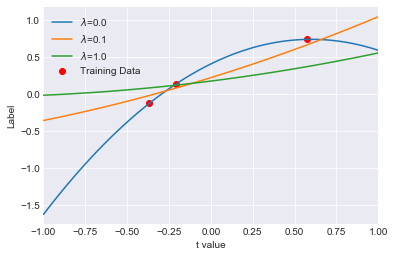
\includegraphics[width=\linewidth]{figures/least_sqaures_prediction.jpg}
    \caption{\textbf{Fitted least squares estimator. } The least squares estimator fitted to the training data (in red) with different values of regularization term.}
    \label{fig:least_squares_with_reg}
\end{figure}

\begin{figure}[t]
    \centering
    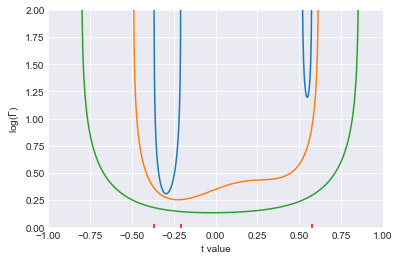
\includegraphics[width=\linewidth]{figures/least_sqaures_regret.jpg}
    \caption{\textbf{PNML regret.} The regret of the PNML predictor from equation \ref{eq:regret} on the interval [-1,1]. The training data t values are marked in red on the x axis.}
    \label{fig:regret_with_reg}
\end{figure}


\section{Conclusions} \label{sec:conclusion}

In this paper we have shown analytic solution for the PNML predictors under the least squares hypothesis class. The mean of that solution is the ERM solution, however, using the PNML, data based uncertainty measure is obtained. In addition we analyzed the space in which the model can be generalize. In addition, we've showed a simulation of least squares polynomial coefficient estimation and the corresponding regret. 
the PNML solution provides an information theoretic learnability
measures that depends on the specic training zN and the specic test features x, may let the
learner know when it does not know.

This work suggests a number of potential directions
for future work. These include: (1) evaluate the PNML predictors for more hypothesis classes. (2) . (3) .


\addtolength{\textheight}{-12cm}   % This command serves to balance the column lengths
                                  % on the last page of the document manually. It shortens
                                  % the textheight of the last page by a suitable amount.
                                  % This command does not take effect until the next page
                                  % so it should come on the page before the last. Make
                                  % sure that you do not shorten the textheight too much.

%%%%%%%%%%%%%%%%%%%%%%%%%%%%%%%%%%%%%%%%%%%%%%%%%%%%%%%%%%%%%%%%%%%%%%%%%%%%%%%%



\bibliographystyle{ieeetr}
\bibliography{refrences.bib}



\end{document}







\end{document}
